\section*{Real ocean microbiome data analysis}

We evaluated the Arc--Hellinger contrast (AHC) on a sparse ocean microbiome data set in which zero handling is not a minor preprocessing detail but a central part of the analysis. The original data contained 180 samples and 23,969 taxa. We focused on the three major water-column layers represented in the metadata: surface water (SRF; $n=83$), deep chlorophyll maximum (DCM; $n=52$), and mesopelagic water (MES; $n=38$), excluding the mixed layer. After retaining taxa observed in at least one of these samples, the analysis included 173 samples and 23,692 taxa. The table was highly sparse: $91.9\%$ of sample-by-taxon entries were zero, with a median library size of 24,482 reads (range: 9,538--45,168). This level of sparsity is precisely the setting in which log-ratio methods must first choose a zero-replacement rule, whereas AHC can be applied directly to the observed closed-simplex compositions.

\subsection*{Alpha diversity}

We first compared AHC-based alpha diversity with Shannon diversity computed under several common zero treatments (Fig.~\ref{fig:ocean-alpha}). For AHC, we used both the geodesic distance from the uniform composition,
\[
D(\pi)=\|\AHC(\pi)\|,
\]
reported on its normalized scale as AHC dominance, and its complementary evenness score,
\[
E(\pi)=1-\frac{D(\pi)}{\arccos(1/\sqrt{p})}.
\]
Because $D$ and $E$ are monotone transformations of the same AHC norm, they give the same omnibus layer test while presenting the result from opposite biological viewpoints.

The AHC alpha index showed a clear layer gradient. AHC dominance decreased from the surface to the mesopelagic layer (mean normalized $D$: SRF $=0.891$, DCM $=0.882$, MES $=0.851$), while AHC evenness increased over the same gradient (mean $E$: SRF $=0.109$, DCM $=0.118$, MES $=0.149$). A one-way ANOVA gave a strong layer effect for both AHC summaries ($F_{2,170}=39.66$, $p=7.31\times 10^{-15}$). Shannon diversity also detected the layer structure when zeros were omitted or when a very small pseudo-count was used (drop-zero Shannon: $F_{2,170}=19.27$, $p=2.85\times 10^{-8}$; pseudo-count $0.01$: $F_{2,170}=18.30$, $p=6.34\times 10^{-8}$). However, the evidence weakened substantially as the pseudo-count increased (pseudo-count $0.5$: $F_{2,170}=3.97$, $p=0.021$) and disappeared at pseudo-count $1$ ($F_{2,170}=2.09$, $p=0.127$).

Thus, the biological pattern was not an artifact introduced by AHC; it was also visible to Shannon when zeros were handled gently. The important difference is that AHC recovered the pattern without requiring a pseudo-count choice, whereas Shannon's apparent layer signal depended on that choice. A Procrustes comparison of the one-dimensional alpha configurations gave high agreement between AHC and drop-zero or small-pseudo-count Shannon ($r=0.94$ and $0.93$, respectively), but substantially lower agreement with Shannon at larger pseudo-counts ($r=0.60$ for pseudo-count $0.5$ and $r=0.49$ for pseudo-count $1$). The alpha analysis therefore illustrates a practical advantage of AHC: it preserves the interpretable layer gradient while removing an otherwise influential tuning parameter.

\begin{figure}[t]
\centering
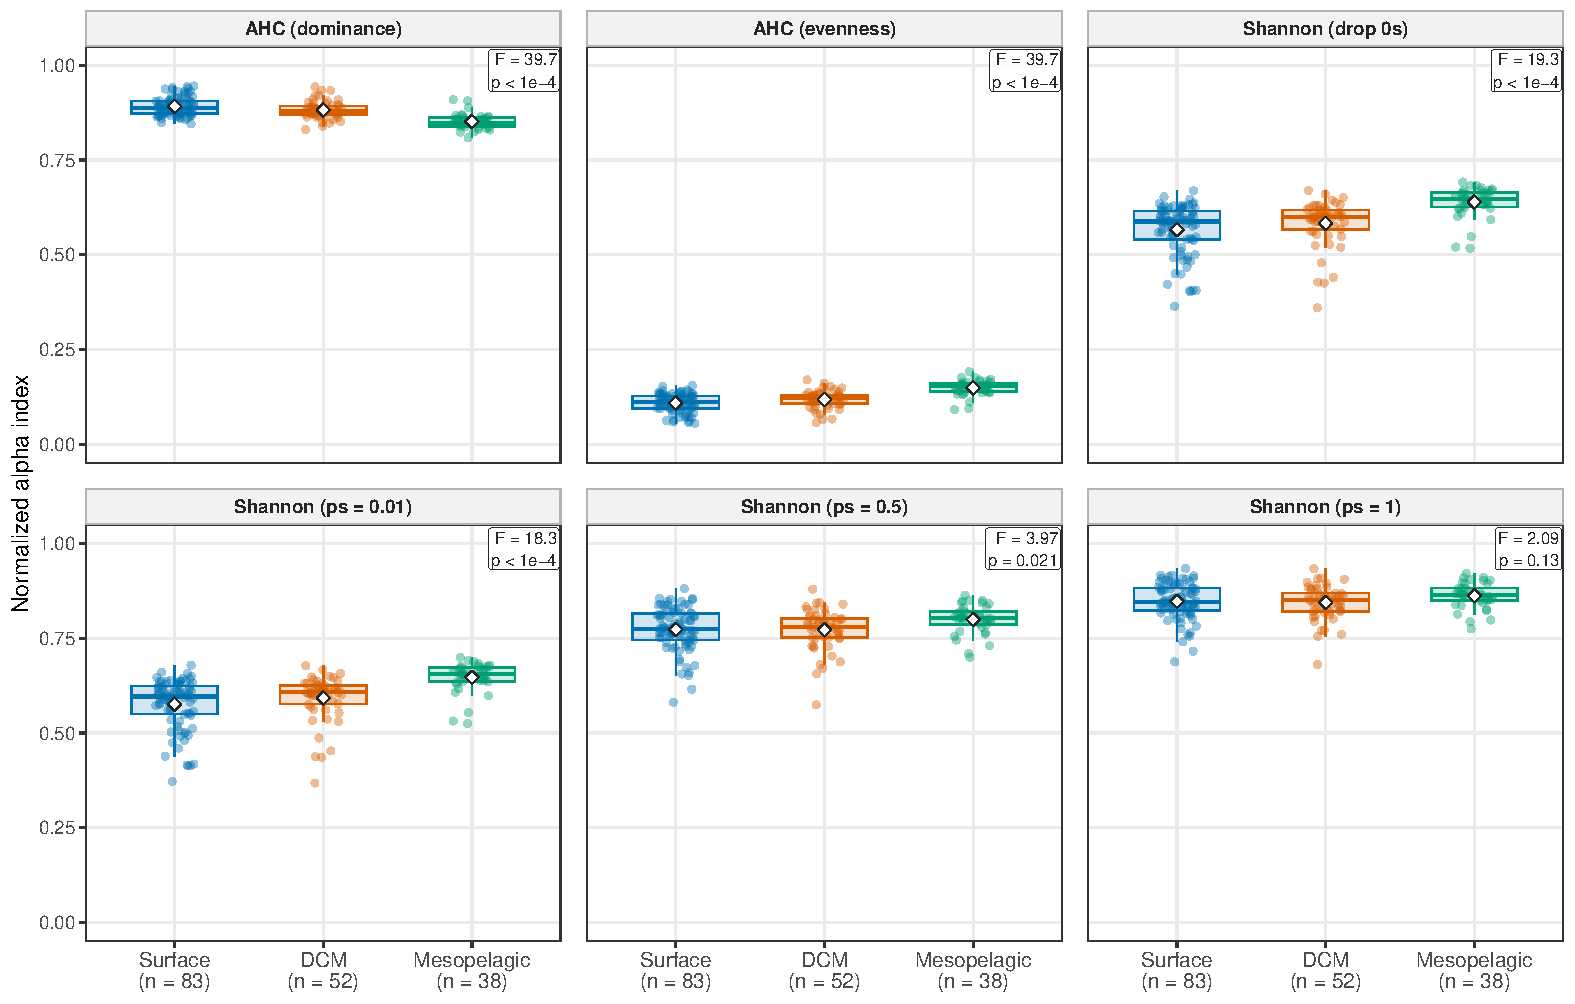
\includegraphics[width=\linewidth]{real_data_ocean_results/figures/fig1_alpha_diversity_by_layer.pdf}
\caption{\textbf{AHC alpha diversity detects the ocean layer gradient without zero replacement.}
Alpha diversity was compared across surface water (SRF; $n=83$), deep chlorophyll maximum (DCM; $n=52$), and mesopelagic water (MES; $n=38$). AHC is shown both as normalized dominance, $D(\pi)/\arccos(1/\sqrt p)$, and as the complementary evenness score, $E(\pi)=1-D(\pi)/\arccos(1/\sqrt p)$. Shannon diversity is shown after dropping zeros and after adding pseudo-counts of $0.01$, $0.5$, and $1$. Points are samples, boxes summarize the layer distributions, and diamonds denote layer means. The upper-right annotation in each panel reports the one-way ANOVA test for a layer effect. AHC gives a strong and pseudo-count-free layer signal, whereas the Shannon result weakens as the pseudo-count increases.}
\label{fig:ocean-alpha}
\end{figure}

\subsection*{Beta diversity}

We next compared the AHC beta diversity,
\[
d_{\AHC}(\pi,\pi')=\|\AHC(\pi)-\AHC(\pi')\|,
\]
with Aitchison distances computed after adding pseudo-counts of $0.01$, $0.5$, or $1$ (Fig.~\ref{fig:ocean-beta}). All four distances separated the three ocean layers in PCoA space, with mesopelagic samples forming the most distinct group and surface and DCM samples showing more partial overlap. PERMANOVA confirmed a strong layer effect for the AHC distance ($R^2=0.147$, $F=14.61$, $p=0.001$). Aitchison distances gave similar but pseudo-count-dependent effect sizes ($R^2=0.144$, $0.176$, and $0.182$ for pseudo-counts $0.01$, $0.5$, and $1$, respectively; all $p=0.001$).

Pairwise PERMANOVA showed that the largest separation involved the mesopelagic layer. Under AHC beta diversity, SRF versus MES had $R^2=0.173$ and DCM versus MES had $R^2=0.169$, whereas SRF versus DCM was much smaller ($R^2=0.029$). This ordering agrees with the visual structure of the ordination and with the expected ecological stratification of the water column. Procrustes analysis further showed that the AHC ordination closely matched the Aitchison ordinations across pseudo-count choices ($r=0.98$ for AHC versus each Aitchison distance). In this data set, AHC therefore preserves the main between-sample geometry obtained from classical log-ratio analysis, while avoiding the need to define unobserved positive values for the $91.9\%$ zero entries.

\begin{figure}[t]
\centering

\includegraphics[width=\linewidth]{real_data_ocean_results/figures/fig2_beta_pcoa_by_method.pdf}
\caption{\textbf{AHC beta diversity recovers the same water-column structure as Aitchison distances without choosing a pseudo-count.}
Principal coordinate analysis was performed using the AHC beta diversity, $d_{\AHC}(\pi,\pi')=\|\AHC(\pi)-\AHC(\pi')\|$, and Aitchison distances computed after pseudo-counts of $0.01$, $0.5$, and $1$. Points are samples and colors indicate ocean layer. Ellipses summarize the layer distributions in each ordination. The annotation in each panel gives the variance explained by the first two PCoA coordinates and the PERMANOVA test for the layer effect. AHC separates surface, DCM, and mesopelagic samples with a structure closely matching the Aitchison ordinations, but it does so directly on the observed sparse compositions.}
\label{fig:ocean-beta}
\end{figure}

\subsection*{Differential abundance}

Finally, we used the transformed coordinates for feature-wise differential abundance testing across layers and compared the resulting taxon sets with CLR-based tests, DESeq2, and LEfSe. To keep the comparison focused on informative taxa, we tested 4,664 taxa after filtering for minimum prevalence and total count. AHC and CLR analyses used one-way ANOVA on transformed feature coordinates, with CLR computed after pseudo-counts of $0.01$, $0.5$, and $1$. DESeq2 was run as an omnibus likelihood-ratio test for the layer effect. Because the LEfSe implementation used here is designed for a dichotomous class variable, we ran one-vs-rest contrasts for each layer and used the union of selected taxa as the LEfSe reference set.

The overall discovery counts were similar but not identical across transformations. AHC identified 3,487 layer-associated taxa, while CLR identified 3,619, 3,692, and 3,690 taxa at pseudo-counts $0.01$, $0.5$, and $1$, respectively. DESeq2 identified 3,171 taxa, and the one-vs-rest LEfSe union contained 1,458 taxa. The overlap structure was more informative than the raw counts (Figs.~\ref{fig:ocean-da-lefse} and \ref{fig:ocean-da-deseq2}). Among the AHC discoveries, 3,337 taxa ($95.7\%$) were also detected by all three CLR pseudo-count analyses, showing that AHC captures the stable core of the transformation-based signal. In the DESeq2 comparison, 2,931 taxa were shared by AHC, all three CLR analyses, and DESeq2; this was the largest intersection and represented $84.1\%$ of all AHC discoveries and $92.4\%$ of all DESeq2 discoveries. Only 6 taxa were unique to AHC in the five-method AHC/CLR/DESeq2 comparison, and only 76 were unique to DESeq2.

The LEfSe comparison told a complementary story. LEfSe selected a smaller reference set, but most of that set was contained in the AHC result: 1,408 of 1,458 LEfSe taxa ($96.6\%$) were also detected by AHC, and 1,370 taxa were shared by AHC, all three CLR pseudo-count analyses, and LEfSe. At the same time, a large group of taxa was consistently detected by AHC and all CLR analyses but not by LEfSe (1,967 taxa), consistent with LEfSe acting as a more selective external reference in this analysis. Taken together, the differential-abundance results show that AHC does not produce an idiosyncratic set of discoveries. Instead, it recovers the main consensus signal across established approaches while making the sensitivity of CLR-based testing to zero replacement explicit.

\begin{figure}[t]
\centering

\includegraphics[width=\linewidth]{real_data_ocean_results/figures/fig3b_da_upset_AHC_CLR_LEfSe.pdf}
\caption{\textbf{AHC differential-abundance discoveries contain the main LEfSe-supported signal while revealing the broader transformation-based consensus.}
The plot summarizes overlap among taxa detected by AHC, CLR after three pseudo-counts, and LEfSe. The left bars show the number of taxa detected by each method. The upper bars show the largest intersections, and the dot matrix indicates which methods contribute to each intersection. LEfSe produced a smaller selected set, but $1,408$ of $1,458$ LEfSe taxa ($96.6\%$) were also detected by AHC; $1,370$ taxa were shared by AHC, all three CLR analyses, and LEfSe. The largest non-LEfSe intersection consisted of taxa detected consistently by AHC and all CLR analyses, illustrating that AHC aligns with the stable transformation-based signal without requiring pseudo-count selection.}
\label{fig:ocean-da-lefse}
\end{figure}

\begin{figure}[t]
\centering

\includegraphics[width=\linewidth]{real_data_ocean_results/figures/fig4b_da_upset_AHC_CLR_DESeq2.pdf}
\caption{\textbf{AHC agrees strongly with the DESeq2-supported consensus set of layer-associated taxa.}
The plot summarizes overlap among taxa detected by AHC, CLR after pseudo-counts of $0.01$, $0.5$, and $1$, and DESeq2. Bar heights show intersection sizes, and the dot matrix identifies the methods represented in each intersection. The largest intersection contains $2,931$ taxa detected by AHC, all three CLR analyses, and DESeq2, accounting for $84.1\%$ of AHC discoveries and $92.4\%$ of DESeq2 discoveries. Method-specific discoveries were small in comparison: only 6 taxa were unique to AHC and 76 were unique to DESeq2 in this five-method comparison.}
\label{fig:ocean-da-deseq2}
\end{figure}

\subsection*{Summary of the real-data analysis}

Across alpha diversity, beta diversity, and differential abundance, the ocean data analysis highlights the practical contribution of AHC. The method is defined directly on the observed sparse compositions, requires no pseudo-count or zero deletion, and nevertheless recovers the same dominant ecological structure seen by established approaches: increasing evenness with depth, strong mesopelagic separation in beta diversity, and a large consensus set of layer-associated taxa. The gain is therefore not merely computational convenience. AHC changes the analysis from one in which zeros must be repaired before standard tools can be used to one in which the boundary of the simplex is part of the modelled sample space. In highly sparse microbiome data, this provides a principled way to obtain stable, interpretable results while still making direct contact with familiar Shannon, Aitchison, DESeq2, and LEfSe analyses.
